\documentclass[12pt]{article}
\usepackage[utf8]{inputenc}
\usepackage{lmodern}
\usepackage[T1]{fontenc}
\usepackage{amsmath}
\usepackage{enumitem}
\usepackage{graphicx}
\usepackage{fullpage}
\usepackage{siunitx}
\usepackage{fancyhdr}
\PassOptionsToPackage{hyphens}{url}
\usepackage[hyphens]{url}
\usepackage{color}
\usepackage{enumitem}
\usepackage{textcomp}
\usepackage{geometry}
\usepackage{courier}
\usepackage{listings}
\usepackage{array}
\usepackage{amsthm}
\usepackage{mathdots}
\usepackage{amssymb}
\usepackage{minted}
\usepackage{wrapfig}
\usepackage{titlesec}
\usepackage{parskip}
\usepackage{accents}
\usepackage{gensymb}
\usepackage{indentfirst}
\usepackage{courier}
\usepackage{framed}
\usepackage{etoolbox}
\usepackage{titlesec}
\usepackage{appendix}
\usepackage{mdframed}
\usepackage{verbatim}
\usepackage{xspace}
\usepackage{hyperref}
\AtBeginEnvironment{subappendices}{%
	\section*{Appendix}
	\addcontentsline{toc}{section}{Appendices}
}

%\lstset{language=C++,
%                basicstyle=\ttfamily,
%                keywordstyle=\color{blue}\ttfamily,
%                stringstyle=\color{red}\ttfamily,
%                commentstyle=\color{green}\ttfamily,
%                morecomment=[l][\color{magenta}]{\#}
%}

\definecolor{keywordcolor}{rgb}{0,0,0.45}
\definecolor{stringcolor}{rgb}{0.45,0.45,0.45}
\definecolor{commentcolor}{rgb}{0,0.3,0}

\lstset{
	language=C++,
	basicstyle=\footnotesize\ttfamily,
	numbers=left,
	%numberstyle=\tiny,
	frame=tb,
	columns=fullflexible,
	showstringspaces=false,
	breaklines=true,
	tabsize=4,
	keywordstyle=\color{keywordcolor}\footnotesize\bf\ttfamily,
	stringstyle=\color{stringcolor}\footnotesize\ttfamily,
	commentstyle=\color{commentcolor}\it\sffamily
}
% \lstset{basicstyle=\ttfamily,breaklines=true}
\lstloadlanguages{C++}

%\renewcommand{\familydefault}{\sfdefault}

\addtolength{\parskip}{\baselineskip}  
\newcommand{\urlwofont}[1]{\urlstyle{same}\url{#1}}

\renewcommand{\arraystretch}{0.8}
\renewcommand{\headrulewidth}{0pt}
\renewcommand{\footrulewidth}{0pt}

\newcommand{\imagewidth}{0.8\textwidth}

\lhead{}
\chead{}
\rhead{}
\lfoot{}
\cfoot{\thepage}
\rfoot{}

\geometry{
	top=0.9in,
	inner=0.7in,
	outer=0.7in,
	bottom=0.9in,
	headheight=2ex,
	headsep=1ex,
}
\pagestyle{fancy}
%\fancyhf{}
%\setlength{\headsep}{0.2in}


\fancypagestyle{firststyle}
{
	\chead{}
	\setlength{\headsep}{0.0in}
}
\hypersetup{
	unicode=true,
	colorlinks=true,
	linkcolor=blue,
	citecolor=black,
	filecolor=black,
	urlcolor=blue
}

\begingroup
\makeatletter
\@for\theoremstyle:=definition,remark,plain\do{%
	\expandafter\g@addto@macro\csname th@\theoremstyle\endcsname{%
		\addtolength\thm@preskip\parskip
	}%
}
\endgroup

\newtheorem{thm}{Theorem}[section]
\newtheorem{lemma}{Lemma}[section]
\newtheorem{claim}{Claim}[section]
\newtheorem{proposition}{Proposition}[section]
%\theoremstyle{empty}
\newtheorem*{namedthm}{Theorem}

% indention size
%\setlength{\parindent}{19pt}
\setlength{\parindent}{0pt}

% paragraph spacing
\setlength{\parskip}{1em}

% line spacing
\linespread{1}

%\setcounter{tocdepth}{1}


% ~~~ Documenting starts here! Please do not change above! ~~~ %

\newcommand{\mytitle}
{
	\textbf {
		inzva Algorithm Programme 2018-2019\\ \ \\
		Bundle 2 \\ \ \\ 
		Algorithms - 1 \\ \ \\
	}
}

\title{\vspace{-2em}\mytitle\vspace{-0.3em}}

\author{
	\textbf{Editor}\\
	Kadir Emre Oto  \\ \ \\ 
	\textbf{Reviewers} \\ 
	Muhammed Burak Buğrul  \\
	Tahsin Enes Kuru
}

\date{}
\begin{document}
	
	\begin{figure}
		\centering
		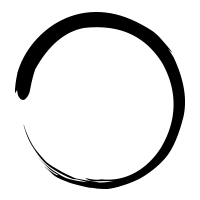
\includegraphics[width=\linewidth/4]{inzva-logo.png}
		\label{fig:inzva}
	\end{figure}
	\maketitle
	
	\cleardoublepage
	\tableofcontents
	\markboth{Table of Contents}{}
	\cleardoublepage
	
	\section{Search Algorithms}
	
It may be necessary to determine if an array or solution set contains a specific data, and we call this finding proccess \textbf{searching}. In this article, three most common search algorithms will be discussed: linear search, binary search, and ternary search.

This visualization may help you understand how the search algorithms work: \href{https://www.cs.usfca.edu/~galles/visualization/Search.html}{Link}. 

		\subsection{Linear Search}
			
Simplest search algorithm is \textit{linear search}, also know as \textit{sequential search}. In this technique, all elements in the collection of the data is checked one by one, if any element matches, algorithm returns the index; otherwise, it returns -1. \\ \\
In the worse case scenario, the search key may not be in the array, or it may be placed towards the end of it. Under these circumstances, the algorithms may check almost all the elements, it means the time complexity is $O(N)$

\begin{figure}[h]
	\centering
	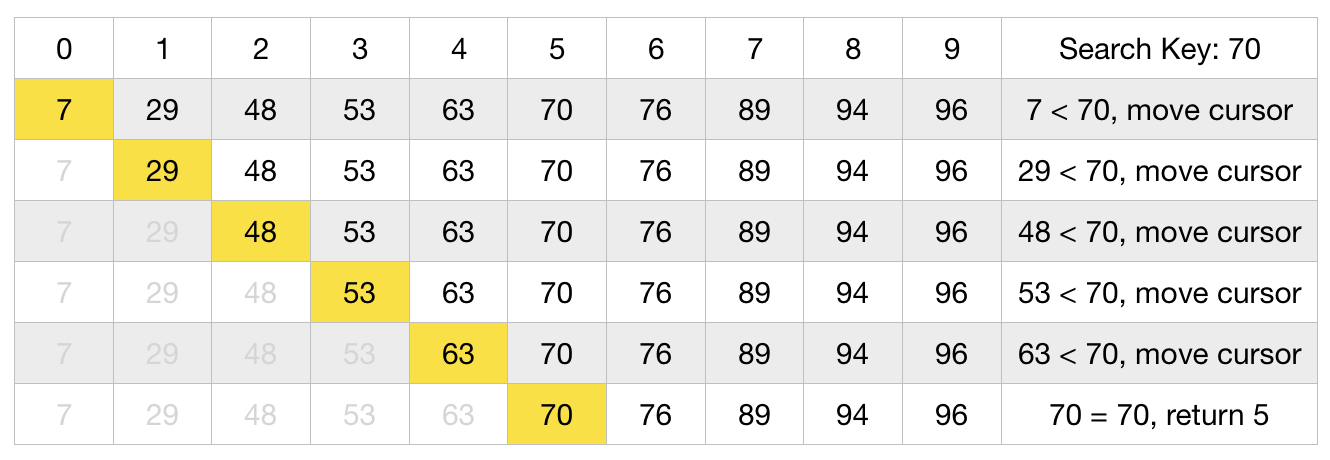
\includegraphics[width=0.9\linewidth]{linear_search}
	\caption{Example for linear search}
	\label{fig:linear_search}
\end{figure}


\begin{minted}[frame=lines,linenos,fontsize=\footnotesize]{c++}
int linearSearch(int *array, int size, int key){
    for (int i=0; i < size; i++)
        if (array[i] == key)
            return i;
    return -1;
}
\end{minted}

\cleardoublepage
	
		\subsection{Binary Search}
			
We know linear search is quite a slow algorithm because it compares each element of the set with search key, and there is a high-speed searching technique for \textbf{sorted} data instead of linear search, which is \textbf{binary search}. After each comparison, the algorithm eliminates half of the data using the sorting property. 

We can also use binary search on increasing functions in the same way. 

\textbf{Procedure: }
\begin{itemize}
	\item Compare the key with the middle element of the array,
	\item If it is a match, return the index of middle.
	\item If the key is bigger than the middle, it means that the key must be in the right side of the middle. We can eliminate the left side.
	\item If the key is smaller, it should be on the left side. The right side can be ignored.
\end{itemize}	

\textbf{Comlexity: }
\begin{eqnarray*}
T(N) &=& T(N / 2) + O(1) \\
T(N) &=& O(logN)
\end{eqnarray*}


\begin{figure}[h]
	\centering
	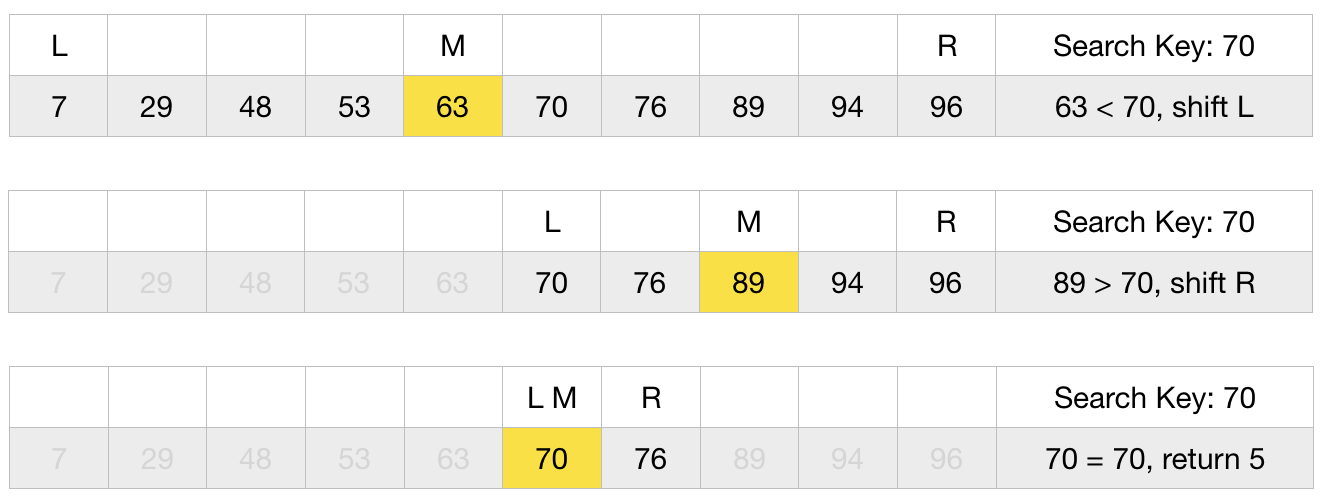
\includegraphics[width=0.9\linewidth]{binary_search}
	\caption{Example for binary search}
	\label{fig:binary_search}
\end{figure}

\cleardoublepage

\begin{minted}[frame=lines,linenos,fontsize=\footnotesize]{c++}
int binarySearch(int *array, int size, int key){
    int left = 0, right = size, mid;

    while (left < right){
        mid = (left + right) / 2;

        if (array[mid] >= key)
            right = mid;
        else
            left = mid + 1;
    }
    return array[left] == key ? left : -1 ;
}
\end{minted}

				\cleardoublepage
		\subsection{Ternary Search}

Suppose that we have a \href{https://www.geeksforgeeks.org/mathematics-unimodal-functions-bimodal-functions/}{unimodal} function, $f(x)$, on an interval $[l, r]$, and we are asked to find the local minimum or the local maximum value of the function according to the behavior of it. \\ \\
There are two types of unimodal functions:

\begin{enumerate}
	\item The function, $f(x)$ strictly increases for $x \leq m$, reaches a global maximum at $x = m$, and then strictly decreases for $m \leq x$. There are no other local maxima.
	
	\item The function, $f(x)$ strictly decreases for $x \leq m$, reaches a global minimum at $x = m$, and then strictly increases for $m \leq x$. There are no other local minima.
\end{enumerate}

In this document, we will implement the first type of unimodal function, and the second one can be solved using the same logic.

\textbf{Procedure: }
\begin{enumerate}
	\item Choose any two points $m_1$, and $m_2$ on the interval $[l, r]$, where $l < m_1 < m_2 < r$.
	\item If $f(m_1) < f(m_2)$, it means the maxima should be in the interval $[m_1, r]$, so we can ignore the interval $[l, m_1]$, move $l$ to $m_1$
	\item Otherwise, $f(m_1) \geq f(m_2)$, the maxima have to be in the interval $[l, m_2]$, move $r$ to $m_2$
	\item If $r - l < \epsilon$, where $\epsilon$ is a negligible value, stop the algorithm, return $l$. Otherwise turn to the step 1. 
\end{enumerate}	

\ \ \ \  $m_1$ and $m_2$ can be selected by $m_1 = l + (r - l) / 3$ and $m_2 = r - (r - l) / 3$ to avoid increasing the time complexity.

\textbf{Comlexity: }
\begin{eqnarray*}
	T(N) &=& T(2 \cdot N / 3) + O(1) \\
	T(N) &=& O(logN)
\end{eqnarray*}



\begin{minted}[frame=lines,linenos,fontsize=\footnotesize]{c++}

double f(double x);

double ternarySearch(double left, double right, double eps=1e-7){
    while (right - left > eps){
        double mid1 = left + (right - left) / 3;
        double mid2 = right - (right - left) / 3;
        
        if (f(mid1) < f(mid2))
            left = mid1;
        else
            right = mid2;
    }
    return f(left);
}
\end{minted}

\cleardoublepage

	\section{Sorting Algorithms}

	
	Sorting algorithms are used to put the elements of an array in a certain order according to the comparison operator. Numerical order or lexcographical orders are the most common ones, and there are a large number of sorting algorithms, but we discuss four of them: \textit{Insertion Sort}, \textit{Merge Sort}, \textit{Quick Sort}, \textit{Radix Sort}. 
	
	For a better understanding, you are strongly recommended to go into this visualization site after reading the topics: \href{https://visualgo.net/en/sorting}{Link}
	
		\subsection{Insertion Sort}
		
Think that you are playing a card game and want to sort them before the game. Your sorting strategy is simple: you have already sorted some part and every time you pick up the next card from unsorted part, you insert it into the correct place in sorted part. After you apply this process to all cards, the whole deck would be sorted. \\ \\
This is the basic idea for sorting an array. We assume that the first element of the array is the sorted part, and other elements are in the unsorted part. Now, we choose the leftmost element of the unsorted part, and put it into the sorted part. In this way the left part of the array always remains sorted after every iteration, and when no element is left in the unsorted part, the array will be sorted. 

	
\begin{minted}[frame=lines,linenos,fontsize=\footnotesize]{c++}
void insertionSort(int *ar, int size){
    for (int i=1; i < size; i++)
        for (int j=i-1; 0 <= j and ar[j] > ar[j+1]; j--)
            swap(ar[j], ar[j+1]);
}
\end{minted}

\cleardoublepage

		\subsection{Merge Sort}

\textit{Merge Sort} is one of the fastest sorting algorithms that uses \textit{Divide and Conquer} paradigm. The algorithm \textbf{divides} the array into two halves, solves each part \textbf{recursively} using same sorting function and \textbf{combines} them in linear time by selecting the smallest value of the arrays every time.

\textbf{Procedure: }
\begin{enumerate}
	\item If the size of the array is 1, it is sorted already, stop the algorithm (base case),
	\item Find the middle point of the array, and split it in two,
	\item Do the algorithm for these parts separately from the first step,
	\item After the two halves got sorted, merge them in linear time and the array will be sorted. 
\end{enumerate}	

\textbf{Comlexity: }
\begin{eqnarray*}
	T(N) &=& T(N / 2) + O(N) \\
	T(N) &=& O(N \cdot logN)
\end{eqnarray*}

\begin{minted}[frame=lines,linenos,fontsize=\footnotesize]{c++}
void mergeSort(int *ar, int size){
    if (size <= 1)  // base case
        return;
	
    mergeSort(ar, size / 2);  // divide the array into two almost equal parts
    mergeSort(ar + size / 2, size - size / 2);
	
    int index = 0, left = 0, right = size / 2;  // merge them 
    int *temp = new int [size];
	
    while (left < size / 2 or right < size){
        if (right == size or (left < size / 2 and ar[left] < ar[right]))
            temp[index++] = ar[left++];
        else 
            temp[index++] = ar[right++];
    }
    for (int i=0; i < size; i++)
        ar[i] = temp[i];
    delete [] temp;
}		
\end{minted}

\cleardoublepage

		\subsection{Quick Sort}
		
\textit{Quick Sort} is also a \textit{Divide and Conquer} algorithm. The algorithm chooses an element from the array as a pivot and partitions the array around it. Partitioning is arranging the array that satisfies those: the pivot should be put to its correct place, all smaller values should be placed before the pivot, and all greater values should be placed after the pivot. The partitioning can be done in linear time, and after the partitioning, we can use the same sorting function to solve the left part of the pivot and the right part of the pivot recursively. \\ \\
If the sellected pivot cannot divide the array uniformly after the partitioning, the time complexity can reach $O(n ^ 2)$ like insertion sort. To avoid this, the pivot can generally be picked randomly.

\textbf{Procedure: }
\begin{enumerate}
	\item If the size of the array is 1, it is sorted already, stop the algorithm (base case),
	\item Choose a pivot randomly,
	\item For all values in the array, collect smaller values in the left of the array and greater values in the right of array,
	\item Move the pivot to the correct place,
	\item Repeat the same algorithm for the left partition and the right partition.
\end{enumerate}	

\textbf{Comlexity: }
\begin{eqnarray*}
	T(N) &=& T(N / 10) + T(9\cdot N / 10) + O(N) \\
	T(N) &=& O(N \cdot logN)
\end{eqnarray*}
		
\begin{minted}[frame=lines,linenos,fontsize=\footnotesize]{c++}
void quickSort(int *ar, int size){
    if (size <= 1)  // base case
        return;
	
    int position = 1;  // find the correct place of pivot
    swap(ar[0], ar[rand() % size]);
	
    for (int i=1; i < size; i++)
        if (ar[0] > ar[i])
            swap(ar[i], ar[position++]);
    swap(ar[0], ar[position-1]);
	
    quickSort(ar, position-1);
    quickSort(ar + position, size - position);
}
\end{minted}

\cleardoublepage
		\subsection{Radix Sort}

	\textit{Quick Sort} and \textit{Merge Sort} are comparison-based sorting algorithms and cannot run better than $O(log N)$. However, \textit{Radix Sort} works in linear time ($O(N + K)$, where $K$ is $log(max(ar))$)).

\textbf{Procedure: }
\begin{enumerate}
	\item For each digit from the least significant to the most, sort the array using \textit{Counting Sort} according to corresponding digit. \textit{Counting Sort} is used for keys between specific range, and it counts the number of elements which have different key values. After counting the number of distict key values, we can determine the position of elements in the array. 
\end{enumerate}	

\textbf{Comlexity: }
\begin{eqnarray*}
	T(N) &=& O(N)
\end{eqnarray*}

\begin{minted}[frame=lines,linenos,fontsize=\footnotesize]{c++}
void radixSort(int *ar, int size, int base=10){
    int *temp = new int [size];
    int *count = new int [base]();
	
    for (int e=1; count[0] != size; e *= base){
        memset(count, 0, sizeof(int) * base);
		
        for (int i=0; i < size; i++)
            count[(ar[i]/e) % base]++;
		
        for (int i=1; i < base; i++)
            count[i] += count[i-1];
		
        if (count[0] == size)
            break;
		
        for (int i=size-1; 0 <= i; i--)
            temp[--count[(ar[i]/e) % base]] = ar[i];
		
        for (int i=0; i < size; i++)
            ar[i] = temp[i];
    }
	
    delete [] temp;
    delete [] count;
}
\end{minted}

\cleardoublepage

	\section{Divide and Conquer}

\textit{Divide and Conquer} is a well-known paradigm that \textbf{breaks} up the problem into several parts, \textbf{solves} each part independently, and finally \textbf{combines} the solutions to the subproblems into the overall solution. Because each subproblem is solved recursively, they should be the smaller versions of the original problem; and the problem must have a base case to end the recursion. 

Some example algorithms that use divide and conquer technique: 
\begin{itemize}
	\item Merge Sort
	\item Count Inversions
	\item Finding the Closest Pair of Points 
	\item \href{https://www.geeksforgeeks.org/divide-and-conquer/}{Others}
\end{itemize}	

\begin{figure}[h]
	\centering
	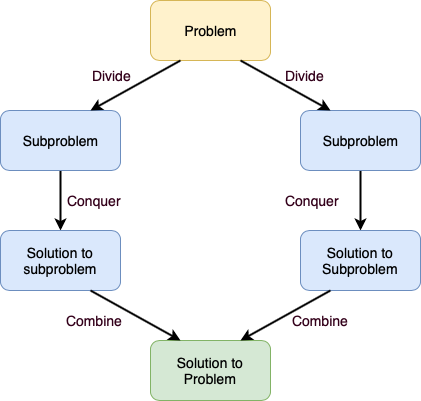
\includegraphics[width=0.55\linewidth]{divide_and_conquer}
	\caption{The Flow of \textit{Divide and Conquer}}
	\label{fig:divide_and_conquer}
\end{figure}


\end{document}
